\section{Implementation of clockless AES}

The AES was written in Balsa in a way that support both Balsa and
Teak simulation and synthesis, avoiding incompatibilites. Focus was at
producing a correct implementation before performance and power, to
demonstrate the feasability of using the tools for relativly
large-scale implementations.

The AES was implemented in an architecture with four 128-bit
registers, two for the data, and two for the key and
key-expansion. Two registers is needed for each, as they are
implemented as single latches and not master/slave latches which does
not, by design, support auto assignments of the form 
$var := var + 1$. The architecture was designed with one control-input,
$instruction$ and two 32-bit data-ports; one for inputp and one for
output. Seven instructions was defined to load, permutate and unload
data from the 128-bit key AES-encryption-circuit.

\begin{description}
  \item[load\_data] Loads 4 32-bit words of data into $reg_0$.
  \item[load\_key128] Loads 4 32-bit words of key into $key_0$.
  \item[add\_key] Sets $reg_1 := reg_0 xor key_0$ (addition in the
    galois field) and then sets $reg_0 := reg_1$ and $key_1 := key_0$.
  \item[sub\_bytes] Calculates $reg_1 := SubBytes(ShiftRows(reg_0))$.
  \item[mix\_col\_expand] Calculates $reg_0 := MixColumns(reg_1)$, and
    $key_0 := ExpandKey(key_1)$.
  \item[skip\_mix\_expand] Only calculates $key_0 := ExpandKey(key_1)$.
  \item[output\_data] Outputs data in $reg_0$ as 4 32-bit words.
\end{description}

To facilitate the testbench, the module aes\_ctrl issues instructions
to the data-path module aes\_data. The source code and corresponding
breeze handshake circuit is shown in figure~\ref{fig:aesctrl}. The
sequence of instructions from aes\_ctrl causes key and plaintext to be
loaded through the input port, encrypted, and then emitted through the
output port. The sourcecode is also shown to illustrate the
straightforwardness of defining sequential behaviour in Balsa and
similar languages.

\begin{figure}[htbp]
  \centering
  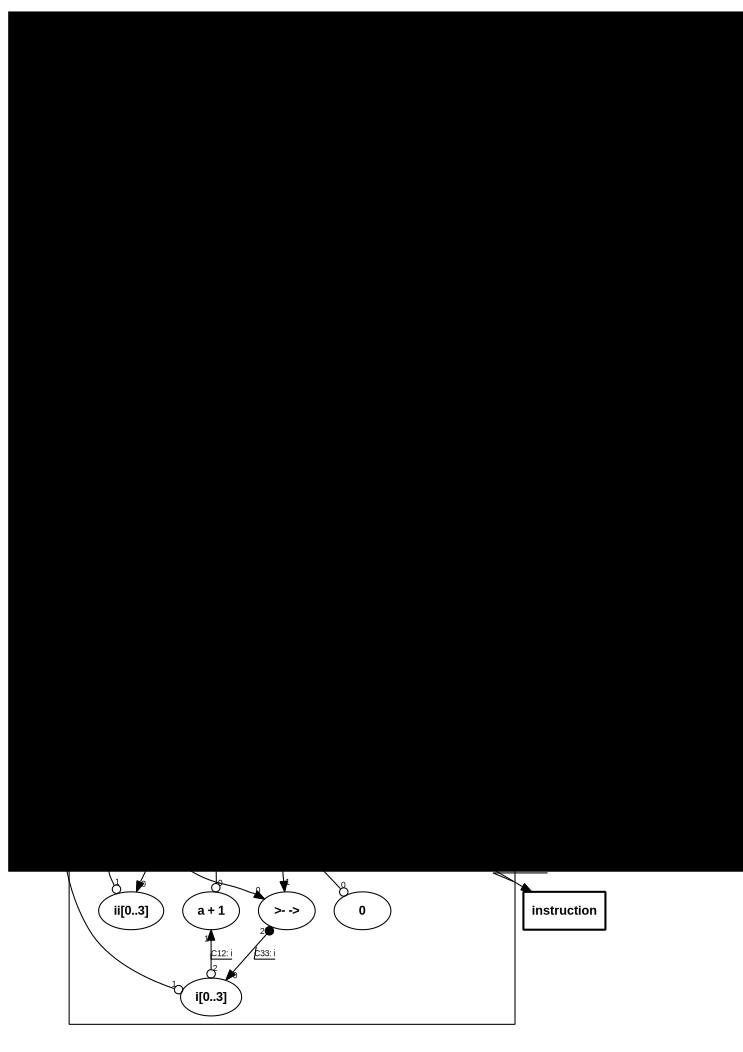
\includegraphics[height=0.9\textheight]{aesctrl.pdf}
  \caption{Source code for AES control module and Balsa handshake
    implementation.}
  \label{fig:aesctrl}
\end{figure}

A 32 bit datapath was chosen for the same reasons given in
\cite{ekelund}, assuming that the same reasoning can be used for
clockless design.

The resources used in the top level design is:
\begin{itemize}
   \item 4 8-bit combinational SubBytes circuits, as as described in
     \cite{combsbox}, shared between the datapath and the keypath.
   \item 1 32-bit mixcolumn circuit employing XXX ``doublers''
   \item 1 128-bit xor-adder circuit
   \item 1 galois field ``doubler'' for the key schedule.
\end{itemize}

The design was designed in Balsa, with frequent compilations to
handshake circuits to visualize what kind of circuit that was
generated. Validation under development was performed using the
behaviroal simulation tool in Balsa, breeze-sim. Each sub-module was
verified for itself, sub-bytes and gfdouble exhaustivly, checking each
of the 256 input output value pairs. The complete AES module was
verified using the NIST testing vectors \cite{nisttest}.


\begin{figure}[htbp]
  \centering
  \includegraphics[height=0.9\textheight]{teaklib.pdf}
  \caption{Library compontents used to synthesize netlists from Balsa
    code with Teak.}
  \label{fig:teaklib}
\end{figure}

While it should be able to implement the breeze handshake circuits to
functionally equivalent netlists for mapping to hardware, I was not
able to do this with the latest version of Balsa\footnote{Balsa 4.0,
  as of this writing, not publicly available, kindly supplied by XXX
  at Manchester University.}, due to missing library files and
documentation. For implementation, I concentrated on using Teak
\cite{teak}, producing netlists consisting of constant delay gates as
shown in figure~\ref{fig:teaklib}.

In addition to the behavrioal simulation, the Verilog netlist
generated from Teak was verified using the GPL version of the verilog
simulation tool cver and again the test-vectors from NIST.
